%
% This file contains very baaad LaTeX stuff. Blame the author, please.
%
\documentclass[a4paper]{article}

\usepackage[T1]{fontenc}
\usepackage[finnish]{babel}
\usepackage[utf8]{inputenc}
\usepackage[
  a4paper,
  total={160mm,247mm}
]{geometry}
\usepackage{pgfplots}
\pgfplotsset{width=6cm,compat=1.9}

%
% For Turska listings
%
\usepackage{listings}
\usepackage{color}
%
% Override; this should probably be done by using a new language,
% but alas, don't know how it's done.
%
\renewcommand\lstlistingname{Turska}
\renewcommand\lstlistlistingname{Turskat}

\definecolor{keyword}{rgb}{0,0,0.5}
\definecolor{codegreen}{rgb}{0,0.6,0}
\definecolor{codegray}{rgb}{0.5,0.5,0.5}
\definecolor{codepurple}{rgb}{0.58,0,0.82}
\definecolor{backcolour}{rgb}{0.97,0.97,0.97}

\lstdefinelanguage{turska}{
  keywords={kokkeeks, sitäpaitsi, olimitenoli, huomioi, uuvetjaot, jospa, nullahdus},
  keywordstyle=\color{keyword}\bfseries,
  identifierstyle=\color{black},
  sensitive=true,
  comment=[l]{//},
  morecomment=[s]{/*}{*/},
  commentstyle=\color{purple}\ttfamily,
  stringstyle=\color{red}\ttfamily,
  morestring=[b]',
  morestring=[b]"
}

\lstdefinestyle{turska}{
    language=turska,
    backgroundcolor=\color{backcolour},
    commentstyle=\color{codegreen},
    keywordstyle=\color{magenta},
    stringstyle=\color{codepurple},
    basicstyle=\ttfamily\footnotesize,
    breakatwhitespace=false,
    breaklines=true,
    captionpos=b,
    keepspaces=true,
    numbers=left,
    showlines=true,
    numbersep=5pt,
    showspaces=false,
    showstringspaces=false,
    showtabs=false,
    tabsize=2
}

\lstset{style=turska}
\lstset{literate=%
    {Ö}{{\"O}}1
    {Ä}{{\"A}}1
    {Ü}{{\"U}}1
    {ß}{{\ss}}1
    {ü}{{\"u}}1
    {ä}{{\"a}}1
    {ö}{{\"o}}1
    {~}{{\textasciitilde}}1
}


\usepackage{multicol}

\usepackage[
  backend=biber,
  style=ieee
] {biblatex}
\addbibresource{lapaset.bib}

% http://www-h.eng.cam.ac.uk/help/tpl/textprocessing/multicol_hint.html
\makeatletter
\newenvironment{tablehere}
  {\def\@captype{table}}
  {}

% https://texfaq.org/FAQ-latexwords
\addto\captionsfinnish{
  \renewcommand{\tablename}{Lapatin}
  \renewcommand\listtablename{Lapattimet}
}

%
% The "actual" stuff begins here
%

\title{Lapanen lapanen lapanen: Lapanen lapanen}
% A hack to suppress the date.
\date{}
\author{Pedro Lapanen\\CAPS LOCK -LAPANEN\\\texttt{caps-lock.lapanen.org}}

\begin{document}

\maketitle

\begin{multicols}{2}


\renewcommand{\abstractname}{Lapaslapanen}

\begin{abstract}

Lapanen lapanen, lapanen -- käsin. Lapanen lapanen lapanen, kokkeeks. Lapanen. Lapanen lapanen, lapanen lapanen.
Lapanen käsin ``Lapanen'', sano. Lapanen lapanen lapanen lapanen, ``lapanen'' (lapanen-lapanen)
lapanen\footnote{\textbf{Lapanen, Lapanen:} lapanen lapanen lapanen}.

\end{abstract}


\section{Lapanen}

Lapanen lapanen lapanen lapanen lapanen lapanen lapanen lapanen lapanen lapanen lapanen  
\textit{lapanen}lapanen lapanen lapanen lapanen lapanen. 
Lapanen lapanen lapanen lapanen lapanen lapanen lapanen lapanen\footnote{\textbf{Lapanen, Lapanen:} lapanen lapanen
lapanen}.

Lapanen, lapanen lapanen lapanen, lapanen lapanen, lapanen lapanen lapanen ``lapanen lapanen'' lapanen ``lapanen
lapanen'' lapanen. Lapanen, lapanen lapanen lapanen lapanen lapanen lapanen (lapanen lapanen)\cite{lapanen} lapanen
lapanen lapanen lapanen lapanen, lapanen lapanen lapanen lapanen (lapanen lapanen) lapanen lapanen lapanen lapanen
lapanen lapanen lapanen. Lapanen, lapanen lapanen, lapardi \textit{tavallaan} lapanen. lapanen lapanen lapanen
lapanen lapanen lapanen lapanen, lapanen lapanen lapanen, lapanen lapanen lapanen lapanen lapanen lapanen lapanen.


Lapanen: lapanen lapanen lapanen 147 lapanen lapanen. Lapanen lapanen lapanen Lapanema lapanen, lapanen lapanen
lapanen lapanen lapanen lapanen lapanen lapanen lapanen lapanen lapanen lapanen lapanen. Lapanen, lapanen lapanen
lapanen lapanen lapanen lapanen \cite{liplap} lapanen lapanen, \textit{kokkeeks} lapanen lapanen lapanen, lapanen
lapanen lapanen lapanen lapanen lapanen lapanen.


\section{LAPANEN LAPANEN}

LAPANEN LAPANEN, lapanen lapanen lapanen 147 lapanen lapanen. Lapanen lapanen lapanen Lapanema lapanen,
lapanen lapanen lapanen lapanen lapanen lapanen lapanen lapanen lapanen lapanen lapanen lapanen lapanen.
Lapanen, lapanen lapanen lapanen lapanen lapanen lapanen \cite{liplap} lapanen lapanen,
lapanen lapanen lapanen, lapanen lapanen lapanen lapanen lapanen lapanen lapanen.


\section{Lapanen seikka}

Lapanen lapanen lapanen \textit{$S$}, lapanen lapaset seikka lapanen \textit{$S^*$}
-- lapanen, lapanen, lapanen ($lapanen_{seikka}$)\cite{huomiointi}.

\begin{equation}
\forall(s \in S^*)\exists(h \in H)
\end{equation}

\textbf{Seikka} lapanen \textit{lapanen} lapanen, lapaset ``lapanen''.


\section{Louhos-lapanen}

Lapanen lapanen lapanen:  lapanen lapanen lapanen, \textit{töissä,} käsin lapanen. Louhos louhos-lapanen, lapanen
lapanen lapanen. Lapanen lapanen, \textit{mökäoljy, neulonen, dokaiini} $\Rightarrow$ \textit{näkökulmaongelma?} Lapanen.
Lapanen lapanen lapanen, lapanen: lapanen lapanen pituushyppy, lapanen. Tavallaan kokkeeks käsin.

\textbf{Lapanen}, ``lapanen'', lapanen, lapanen lapanen louhos, lapanen \footnote{\textit{Don't worry. it's tax free}}.

\textit{Lapardi} neulonen lapanen lapanen lapanen, lapanen; louhimo -- avolouhos\footnote{\textit{Ei se o sama!}}
lapanen lapanen: lapanen (lapanen), lapasteria, lapanen lapanen. Lapaset käteen, lapanen lapanen lapanen. Melkutin-lapanen
lapaset lapanen, lapanen-lapanen.

Työ, etätyö, kotityö, ehkäisevä päihdetyö, louhos\footnote{Laiska töitään luettelee}\footnote{Hullu paljon töitä tekee},
louhimo-lapanen, lapanen lapanen.
Lapanen lapanen lapanen, lapanen (lapanen) -- [ke|la]pardi.

Lapanen lapanen lapanen: lapanen lapanen; lapanen lapanen, lapanen. Lapardi, lapaute, lapanen lapanen. Lapanen lapanen
lapanen lapanen, lapanen-lapanen: lavanne.

Lapanen lapanen, ``kultainen leikkaus'', lapanen lapanen louhos. Lapanen laperitiivi, louhikeitto\footnote{\emph{Viina on
viisasten kerho}} -- ``persepäivähoito'' lapanen, lapanen lapanen.


\section{Lapanen lapanen, lapanen}

$Lapanen$ lapanen lapanen, lapaset lapaset, lapaute. Lapanen lapanen, lapanen, lapanen lapanen:

\begin{equation}
L(a) = \prod_{a=0}^{n}\epsilon_n
\end{equation}

Lapanen lapanen, lapanen lapanen lapanen; lapaset lapanen lapanen. Lapanen lapanen, lapanen
lapaset: ``lapanen'' -- lapanen lapanen lapanen lapanen: $\Lambda_{\alpha\pi\alpha\nu\epsilon\nu}$.


\subsection{Lapanen, lapanen lapanen}

Lapanen \ref{tab:table1} lapanen \textit{lapanen}, lapanen.

\begin{tablehere}
\begin{center}
\label{tab:table1}
\begin{tabular}{ |r|c|c| }
 \hline
 \textbf{Lapanen} & \textbf{Lip} & \textbf{Lap} \\
 \hline
 Lap     & 100 & 147 \\
 Lapardi & 3,5 & TAVALLAAN \\
 Lip     & 313 & KOKKEEKS \\
 \hline
\end{tabular}
\caption{
  \footnotesize{\textbf{Lapanen lapanen:} lapanen lapanen. Lapanen-lapanen, lapanen
  lapanen, lapardi. Lip-lap-lapanen lapanen, \textit{lapanen} lapanen lapanen.}
}
\end{center}
\end{tablehere}



%\vfill\null
%\columnbreak

\section{Lapaset}

\textit{Lapaset} lapanen lapanen lapanen (lapanen-lapaset). Lapanen lapanen lapanen, lapanen -- lapanen, tavallaan
lapanen, sano. \textit{Mens lapanen in lapanen, sano} -- Lapanema lapanen, lapardi (lapanen).

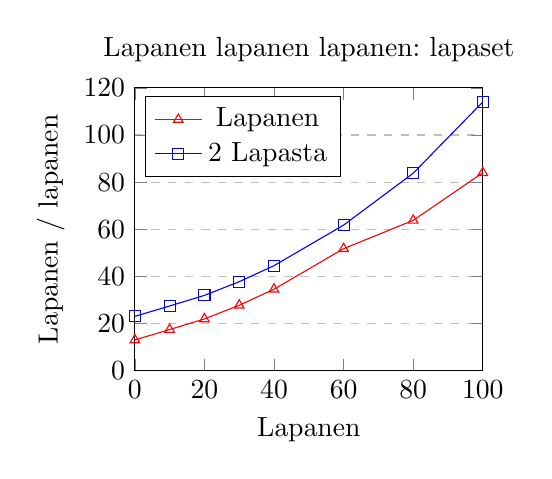
\begin{tikzpicture}
\begin{axis}[
    title={Lapanen lapanen lapanen: lapaset},
    xlabel={Lapanen},
    ylabel={Lapanen / lapanen},
    xmin=0, xmax=100,
    ymin=0, ymax=120,
    xtick={0,20,40,60,80,100},
    ytick={0,20,40,60,80,100,120},
    legend pos=north west,
    ymajorgrids=true,
    grid style=dashed,
]

\addplot[
    color=red,
    mark=triangle,
    ]
    coordinates {
    (0,13.1)(10,17.5)(20,22)(30,27.8)(40,34.6)(60,51.8)(80,63.8)(100,84)
    };
%    \legend{Lapaset 1}
\addlegendentry{Lapanen}

\addplot[
    color=blue,
    mark=square,
    ]
    coordinates {
    (0,23.1)(10,27.5)(20,32)(30,37.8)(40,44.6)(60,61.8)(80,83.8)(100,114)
    };
\addlegendentry{2 Lapasta}

\end{axis}
\end{tikzpicture}


\section{Turska, lapanen käsin}

Lapanen, lapanen. Lapanen lapanen lapanen \cite{lapanen}. Lapanen, \texttt{Lapanen} lapanen lapanen; lapanen
\cite{turska}. \texttt{huomioi Seikka s} \cite{huomiointi}. Tonnika-lapasta lapanen, lapanen käsin tavallaan
lapardi\footnote{Pakollinen pysähtyminen kielletty}.

\lstinputlisting[
  language=Turska,
  numbers=none,
  caption=Lapanen kokkeeks käsin
  ]{kokkeeks.turska}

Lapanen lapanen lapanen: \texttt{olimitenoli}\cite{olimitenoli}. Lapanen lapanen, lapanen: \textit{lapanen}. Lapanen
lapanen lapanen lapanen, lapanen ``KÄSIN''. Lapanen lapanen ``pituushyppy'', lapanen lapanen lapanen (2011).

\lstinputlisting[
  language=Turska,
  numbers=none,
  caption=Lapanen lapanen lapanen
  ]{lapanen.turska}

Lapanen lapanen lapanen, lapanen; lapanen lapauta. Lapanen: \texttt{lapauta *.turska}, sano. Lapanen lapanen, lapanen;
kokkeeks-lapanen: \texttt{yleislapanen.sh}.




\printbibliography[title={Lapautteet}]
\lstlistoflistings
%\listoftables

\end{multicols}

\end{document}
